

\begin{wrapfigure}[0]{r}[-2cm]{4cm}
 \vspace{-5cm}
 %\centering 
 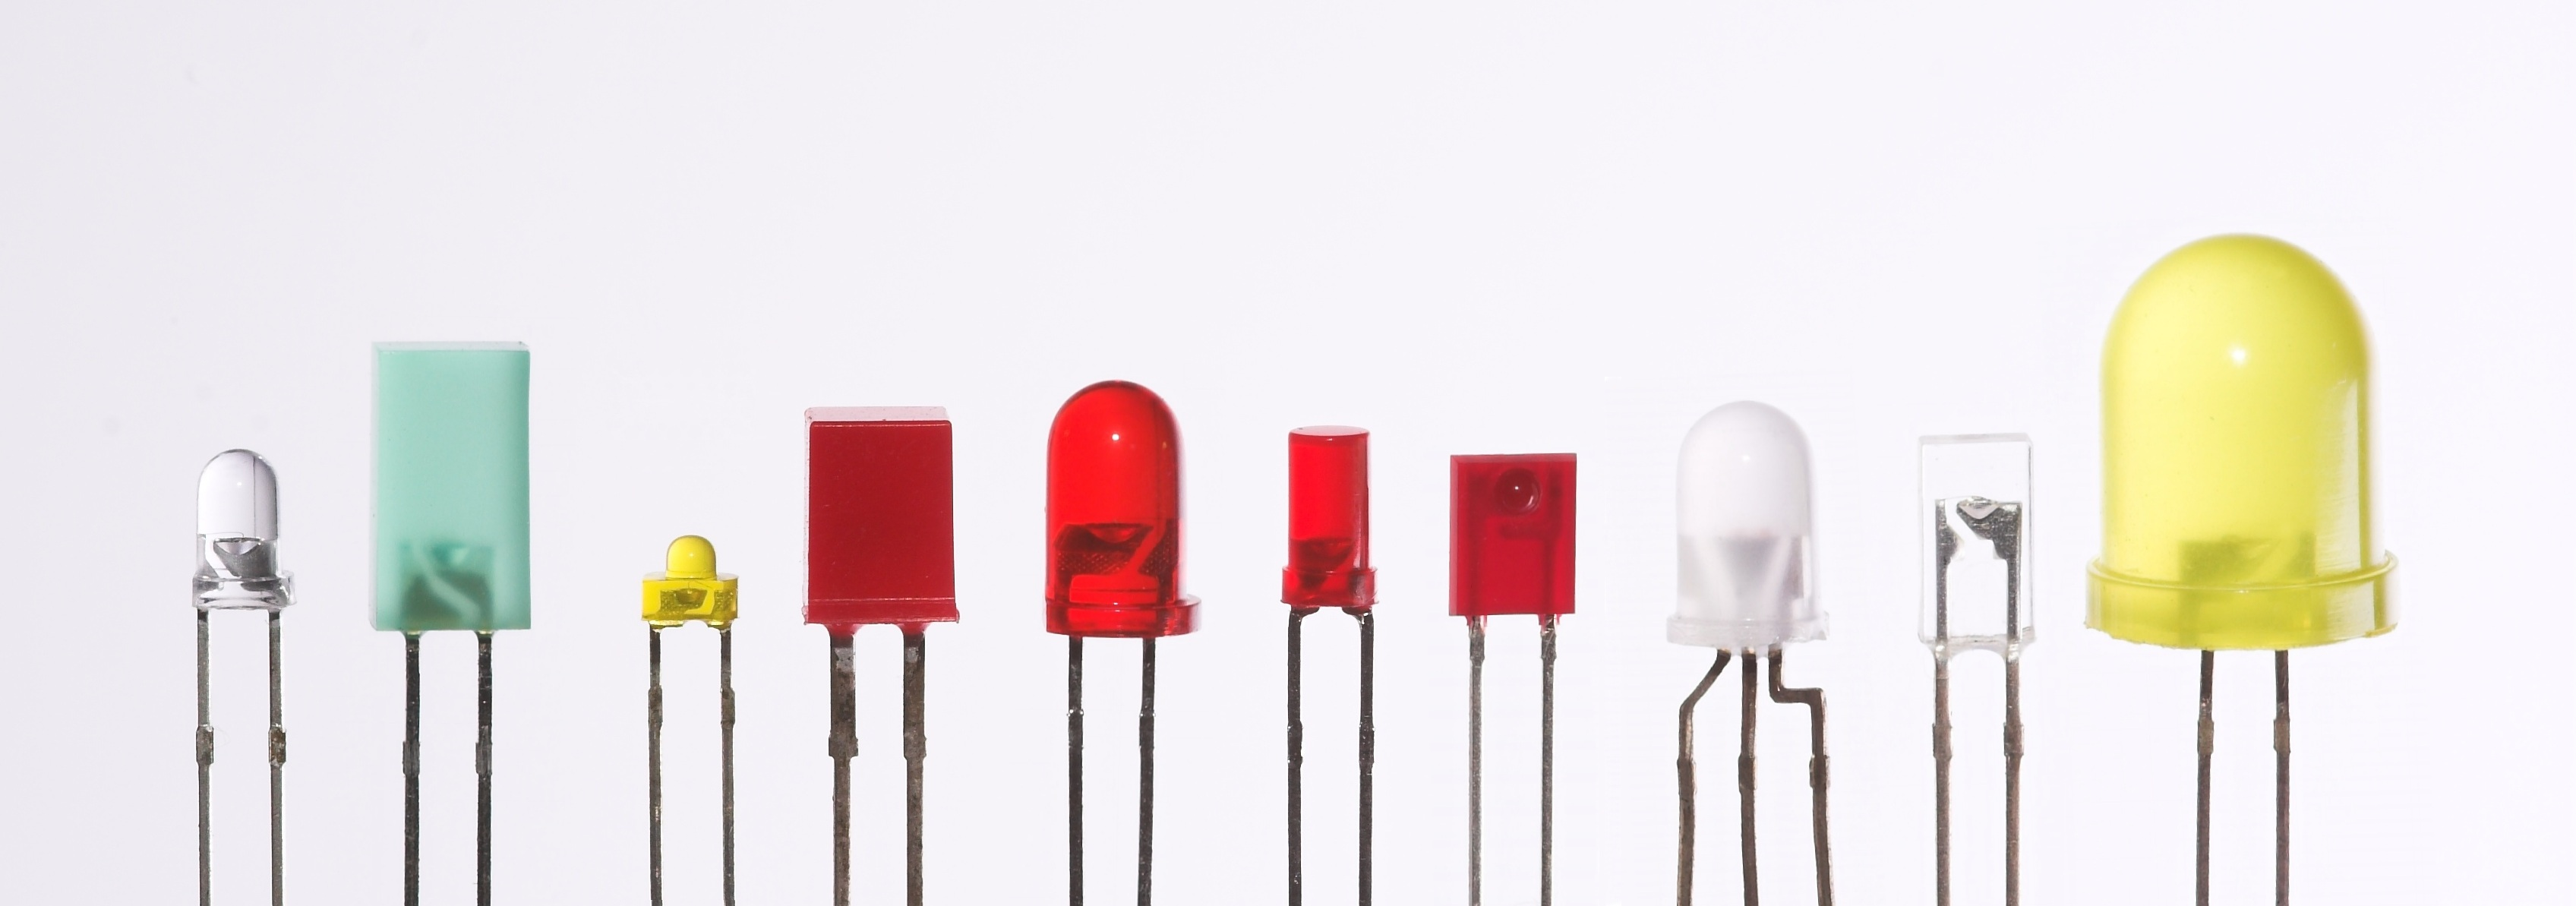
\includegraphics[scale=0.25]{Diode/Bilder/Verschiedene_LEDs.jpg}
 %\caption{Bildunterschrift der Grafik.}
 %\label{fig:meine-Grafik}
 \vspace*{-5cm}
\end{wrapfigure}


\section*{Theorie- und Prüfungsfragen} 

\subsection*{Dotierung}

\begin{enumerate}
	\itemsep1pt\parskip0pt\parsep0pt
	\item[1] Was bedeutet der Begriff Dotierung?
        \loesung{\textbf{Dotierung} bezeichnet in der Halbleitertechnik das
        einbringen von Fremdatomen in ein Grundmaterial zur Veränderung der
        elektrischen Leitfähigkeit.}
\end{enumerate}

\begin{enumerate}
\item[2] \emph{\textbf{TB105}}    Was verstehen Sie unter Halbleitermaterialien? Einige Stoffe wie z.B. ...
	\begin{enumerate}
	\itemsep1pt\parskip0pt\parsep0pt
		\item[A] Silizium, Germanium sind in reinem Zustand gute Isolatoren. Durch geringfügige Zusätze von geeigneten anderen Stoffen werden sie jedoch zu Leitern.
		\item[B] Silizium, Germanium sind in reinem Zustand gute Isolatoren. Durch geringfügige Zusätze von geeigneten anderen Stoffen nimmt jedoch ihre Leitfähigkeit ab.
		\item[C]  Indium oder Magnesium sind in reinem Zustand gute Isolatoren. Durch geringfügige Zusätze von geeigneten anderen Stoffen werden sie jedoch zu Leitern.
		\item[D] Silizium, Germanium sind in trockenem Zustand gute Elektrolyten. Durch geringfügige Zusätze von Wismut oder Tellur kann man daraus entweder N-leitendes oder P-leitendes Material für Anoden bzw. Katoden von Halbleiterbauelementen herstellen.
		\loesung{Lösung A}
	\end{enumerate}
\end{enumerate}

\begin{enumerate}
\item[3] \emph{\textbf{TC501}}    P-dotiertes Halbleitermaterial ist solches, das mit einem zusätzlichen Stoff versehen wurde, der
	\begin{enumerate}
	\itemsep1pt\parskip0pt\parsep0pt
		\item[A] mehr als vier Valenzelektronen enthält.
		\item[B] genau vier Valenzelektronen enthält.
		\item[C] weniger als vier Valenzelektronen enthält.
		\item[D] keine Valenzelektronen enthält.
		 \loesung{Lösung C}
	\end{enumerate}
\end{enumerate}


\begin{enumerate}
\item[4] \emph{\textbf{TC502}}   N-leitendes Halbleitermaterial ist gekennzeichnet durch
	\begin{enumerate}
	\itemsep1pt\parskip0pt\parsep0pt
		\item[A] Überschuss an freien Elektronen.
		\item[B] das Fehlen von Dotierungsatomen.
		\item[C] das Fehlen von Atomen im Gitter des Halbleiterkristalls.
		\item[D] bewegliche Elektronenlücken.
		\loesung{Lösung A}
	\end{enumerate}
\end{enumerate}


\begin{enumerate}
\item[5] \emph{\textbf{TC503}}  Ein in Durchlassrichtung betriebener PN-Übergang ermöglicht
	\begin{enumerate}
	\itemsep1pt\parskip0pt\parsep0pt
		\item[A] den Stromfluss von N nach P.
		\item[B] den Stromfluss von P nach N.
		\item[C] keinen Stromfluss.
		\item[D] den Elektronenfluss von P nach N.
		\loesung{Lösung B}
	\end{enumerate}
\end{enumerate}


\subsection*{Die Diode}

\begin{enumerate}
\itemsep1pt\parskip0pt\parsep0pt
\item[6] Skizziere das Schaltzeichen einer Diode und markiere die Anode, die Kathode und die jeweilige Dotierung.
    \loesung{
    \begin{figure}[H]
    \centering 
    % Graphic for TeX using PGF
% Title: /home/stole/Dokumente/git/afutub-kurs/Praxisskript/Diode/Schaltungen/Diode.dia
% Creator: Dia v0.97.3
% CreationDate: Mon Nov 16 20:36:17 2015
% For: stole
% \usepackage{tikz}
% The following commands are not supported in PSTricks at present
% We define them conditionally, so when they are implemented,
% this pgf file will use them.
\ifx\du\undefined
  \newlength{\du}
\fi
\setlength{\du}{15\unitlength}
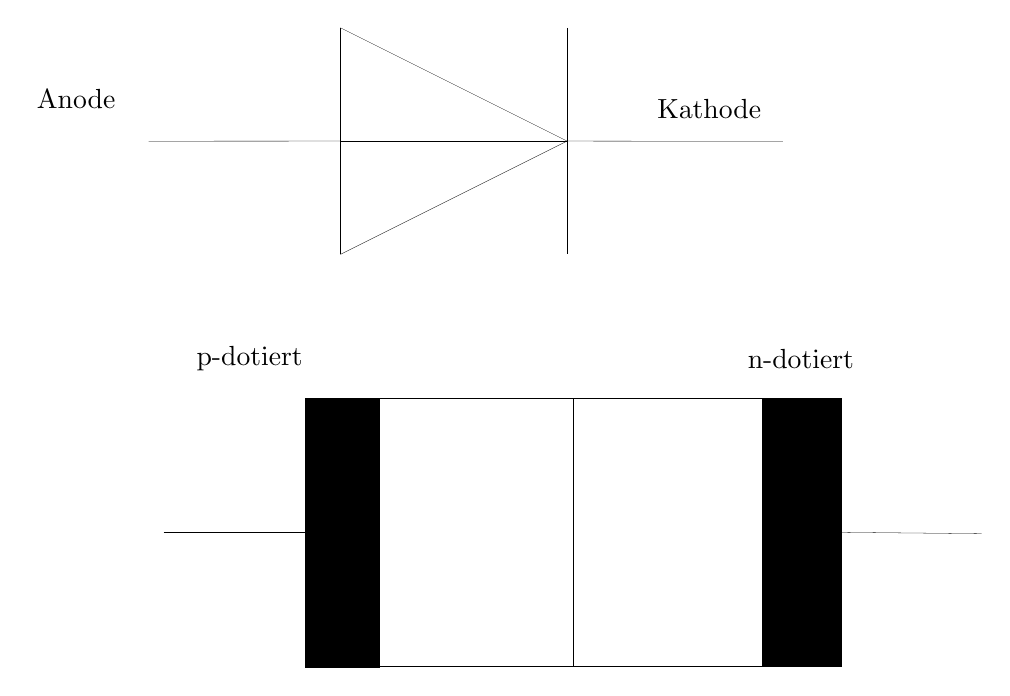
\begin{tikzpicture}
\pgftransformxscale{1.000000}
\pgftransformyscale{-1.000000}
\definecolor{dialinecolor}{rgb}{0.000000, 0.000000, 0.000000}
\pgfsetstrokecolor{dialinecolor}
\definecolor{dialinecolor}{rgb}{1.000000, 1.000000, 1.000000}
\pgfsetfillcolor{dialinecolor}
\pgfsetlinewidth{0.100000\du}
\pgfsetdash{}{0pt}
\pgfsetdash{}{0pt}
\pgfsetbuttcap
\pgfsetmiterjoin
\pgfsetbuttcap
\pgfsetmiterjoin
\pgfsetdash{}{0pt}
\definecolor{dialinecolor}{rgb}{0.000000, 0.000000, 0.000000}
\pgfsetstrokecolor{dialinecolor}
\draw (15.422302\du,-15.899999\du)--(15.422302\du,-13.022298\du);
\pgfsetbuttcap
\pgfsetmiterjoin
\pgfsetdash{}{0pt}
\definecolor{dialinecolor}{rgb}{0.000000, 0.000000, 0.000000}
\pgfsetstrokecolor{dialinecolor}
\draw (15.422302\du,-13.022298\du)--(18.300002\du,-14.461149\du);
\pgfsetbuttcap
\pgfsetmiterjoin
\pgfsetdash{}{0pt}
\definecolor{dialinecolor}{rgb}{0.000000, 0.000000, 0.000000}
\pgfsetstrokecolor{dialinecolor}
\draw (15.422302\du,-15.899999\du)--(18.300002\du,-14.461149\du);
\pgfsetbuttcap
\pgfsetmiterjoin
\pgfsetdash{}{0pt}
\definecolor{dialinecolor}{rgb}{0.000000, 0.000000, 0.000000}
\pgfsetstrokecolor{dialinecolor}
\draw (15.422302\du,-14.461149\du)--(18.300002\du,-14.461149\du);
\pgfsetbuttcap
\pgfsetmiterjoin
\pgfsetdash{}{0pt}
\definecolor{dialinecolor}{rgb}{0.000000, 0.000000, 0.000000}
\pgfsetstrokecolor{dialinecolor}
\draw (18.300002\du,-15.899999\du)--(18.300002\du,-13.022298\du);
\pgfsetlinewidth{0.100000\du}
\pgfsetdash{}{0pt}
\pgfsetdash{}{0pt}
\pgfsetbuttcap
{
\definecolor{dialinecolor}{rgb}{0.000000, 0.000000, 0.000000}
\pgfsetfillcolor{dialinecolor}
% was here!!!
\definecolor{dialinecolor}{rgb}{0.000000, 0.000000, 0.000000}
\pgfsetstrokecolor{dialinecolor}
\draw (18.300002\du,-14.461149\du)--(21.040301\du,-14.459230\du);
}
\pgfsetlinewidth{0.100000\du}
\pgfsetdash{}{0pt}
\pgfsetdash{}{0pt}
\pgfsetbuttcap
{
\definecolor{dialinecolor}{rgb}{0.000000, 0.000000, 0.000000}
\pgfsetfillcolor{dialinecolor}
% was here!!!
\definecolor{dialinecolor}{rgb}{0.000000, 0.000000, 0.000000}
\pgfsetstrokecolor{dialinecolor}
\draw (12.987653\du,-14.460276\du)--(15.422302\du,-14.461149\du);
}
% setfont left to latex
\definecolor{dialinecolor}{rgb}{0.000000, 0.000000, 0.000000}
\pgfsetstrokecolor{dialinecolor}
\node[anchor=west] at (11.448825\du,-14.995418\du){Anode};
% setfont left to latex
\definecolor{dialinecolor}{rgb}{0.000000, 0.000000, 0.000000}
\pgfsetstrokecolor{dialinecolor}
\node[anchor=west] at (19.327825\du,-14.872736\du){Kathode};
\pgfsetlinewidth{0.100000\du}
\pgfsetdash{}{0pt}
\pgfsetdash{}{0pt}
\pgfsetmiterjoin
\definecolor{dialinecolor}{rgb}{1.000000, 1.000000, 1.000000}
\pgfsetfillcolor{dialinecolor}
\fill (14.976770\du,-11.192971\du)--(14.976770\du,-7.792972\du)--(18.376770\du,-7.792972\du)--(18.376770\du,-11.192971\du)--cycle;
\definecolor{dialinecolor}{rgb}{0.000000, 0.000000, 0.000000}
\pgfsetstrokecolor{dialinecolor}
\draw (14.976770\du,-11.192971\du)--(14.976770\du,-7.792972\du)--(18.376770\du,-7.792972\du)--(18.376770\du,-11.192971\du)--cycle;
\pgfsetlinewidth{0.100000\du}
\pgfsetdash{}{0pt}
\pgfsetdash{}{0pt}
\pgfsetmiterjoin
\definecolor{dialinecolor}{rgb}{1.000000, 1.000000, 1.000000}
\pgfsetfillcolor{dialinecolor}
\fill (18.376770\du,-11.192970\du)--(18.376770\du,-7.792971\du)--(21.776770\du,-7.792971\du)--(21.776770\du,-11.192970\du)--cycle;
\definecolor{dialinecolor}{rgb}{0.000000, 0.000000, 0.000000}
\pgfsetstrokecolor{dialinecolor}
\draw (18.376770\du,-11.192970\du)--(18.376770\du,-7.792971\du)--(21.776770\du,-7.792971\du)--(21.776770\du,-11.192970\du)--cycle;
\pgfsetlinewidth{0.100000\du}
\pgfsetdash{}{0pt}
\pgfsetdash{}{0pt}
\pgfsetbuttcap
{
\definecolor{dialinecolor}{rgb}{0.000000, 0.000000, 0.000000}
\pgfsetfillcolor{dialinecolor}
% was here!!!
\definecolor{dialinecolor}{rgb}{0.000000, 0.000000, 0.000000}
\pgfsetstrokecolor{dialinecolor}
\draw (13.176770\du,-9.492971\du)--(14.976770\du,-9.492972\du);
}
\pgfsetlinewidth{0.100000\du}
\pgfsetdash{}{0pt}
\pgfsetdash{}{0pt}
\pgfsetmiterjoin
\definecolor{dialinecolor}{rgb}{0.000000, 0.000000, 0.000000}
\pgfsetfillcolor{dialinecolor}
\fill (14.976770\du,-11.192971\du)--(14.976770\du,-7.778107\du)--(15.911899\du,-7.778107\du)--(15.911899\du,-11.192971\du)--cycle;
\definecolor{dialinecolor}{rgb}{0.000000, 0.000000, 0.000000}
\pgfsetstrokecolor{dialinecolor}
\draw (14.976770\du,-11.192971\du)--(14.976770\du,-7.778107\du)--(15.911899\du,-7.778107\du)--(15.911899\du,-11.192971\du)--cycle;
\pgfsetlinewidth{0.100000\du}
\pgfsetdash{}{0pt}
\pgfsetdash{}{0pt}
\pgfsetmiterjoin
\definecolor{dialinecolor}{rgb}{0.000000, 0.000000, 0.000000}
\pgfsetfillcolor{dialinecolor}
\fill (20.776770\du,-11.192971\du)--(20.776770\du,-7.792971\du)--(21.776770\du,-7.792971\du)--(21.776770\du,-11.192971\du)--cycle;
\definecolor{dialinecolor}{rgb}{0.000000, 0.000000, 0.000000}
\pgfsetstrokecolor{dialinecolor}
\draw (20.776770\du,-11.192971\du)--(20.776770\du,-7.792971\du)--(21.776770\du,-7.792971\du)--(21.776770\du,-11.192971\du)--cycle;
% setfont left to latex
\definecolor{dialinecolor}{rgb}{0.000000, 0.000000, 0.000000}
\pgfsetstrokecolor{dialinecolor}
\node[anchor=west] at (13.476772\du,-11.692970\du){p-dotiert};
% setfont left to latex
\definecolor{dialinecolor}{rgb}{0.000000, 0.000000, 0.000000}
\pgfsetstrokecolor{dialinecolor}
\node[anchor=west] at (20.476772\du,-11.692970\du){n-dotiert};
\pgfsetlinewidth{0.100000\du}
\pgfsetdash{}{0pt}
\pgfsetdash{}{0pt}
\pgfsetbuttcap
{
\definecolor{dialinecolor}{rgb}{0.000000, 0.000000, 0.000000}
\pgfsetfillcolor{dialinecolor}
% was here!!!
\definecolor{dialinecolor}{rgb}{0.000000, 0.000000, 0.000000}
\pgfsetstrokecolor{dialinecolor}
\draw (21.776770\du,-9.492971\du)--(23.565624\du,-9.475251\du);
}
\end{tikzpicture}

    \end{figure}
    }
\item[7] Skizziere die Strom-Spannungskennlinie und markieren den Durchlassbereich, den Sperrbereich und den Durchbruchbereich.
	\loesung{
	\begin{figure}[H]
    \centering 
    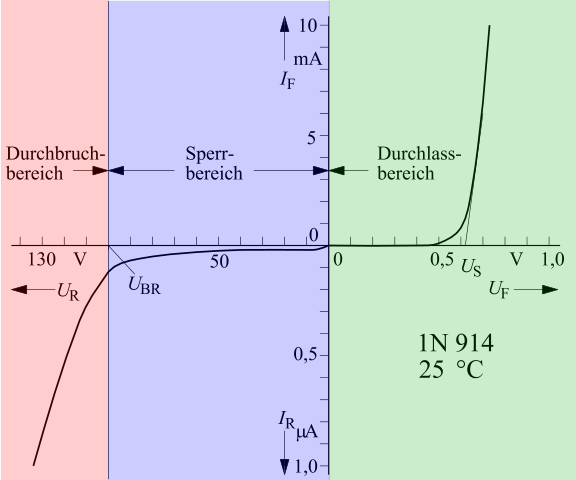
\includegraphics[scale=0.5]{Diode/Bilder/Kennlinie_Diode.png}
    \end{figure}
    }

\mucho{8}{TC504}
{Eine in Sperrrichtung betriebene Diode hat}%Frage
{einen hohen Widerstand.}%A
{eine hohe Kapazität.}%B
{eine geringe Impedanz.}%C
{eine hohe Induktivität.}%D
{A}%Lösung

\mucho{9}{TC508}
{Wozu dient die folgende Schaltung?\\ 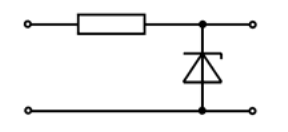
\includegraphics[scale=0.63]{Diode/Bilder/TC508.png}}%Frage
{zur Signalbegrenzung.}%A
{zur Spannungsstabilisierung.}%B
{als Leuchtanzeige.}%C
{zur Stromgewinnung.}%D
{B}%Lösung

\mucho{10}{TC505}
{Die Auswahlantworten enthalten Silizium-Dioden mit unterschiedlichen Arbeitspunkten. Bei welcher Antwort befindet sich die Diode in leitendem Zustand?}%Frage
{$-2,6V $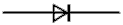
\includegraphics[scale=0.5]{Diode/Bilder/Diode_r.png} $-2,0V$}%A
{$~~~~15V$ 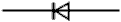
\includegraphics[scale=0.5]{Diode/Bilder/Diode_l.png} $~~~9V$}%B
{$~~0,7V$ 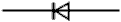
\includegraphics[scale=0.5]{Diode/Bilder/Diode_l.png} $1,3V$}%C
{$~~3,4V$ 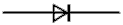
\includegraphics[scale=0.5]{Diode/Bilder/Diode_r.png} $4,0V$}%D
{C}%Lösung

\mucho{11}{TC506}
{Die Auswahlantworten enthalten Silizium-Dioden mit unterschiedlichen Arbeitspunkten. Bei welcher Antwort befindet sich die Diode in leitendem Zustand?}%Frage
{$~~5,3V $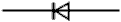
\includegraphics[scale=0.5]{Diode/Bilder/Diode_l.png} $4,7V$}%A
{$~~15V$ 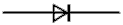
\includegraphics[scale=0.5]{Diode/Bilder/Diode_r.png} $18V$}%B
{$3,9V$ 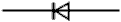
\includegraphics[scale=0.5]{Diode/Bilder/Diode_l.png} $3,2V$}%C
{$-2V$ 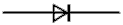
\includegraphics[scale=0.5]{Diode/Bilder/Diode_r.png} $-2,6V$}%D
{D}%Lösung

\mucho{12}{TC509}
{Wozu dient die folgende Schaltung?\\ 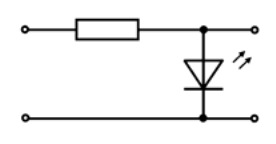
\includegraphics[scale=0.63]{Diode/Bilder/TC509.png}}%Frage
{zur Signalbegrenzung.}%A
{als Leuchtanzeige.}%B
{zur Stromgewinnung.}%C
{zur Spannungsstabilisierung.}%D
{B}%Lösung

\mucho{13}{TC507}
{Wie verhält sich die Kapazität einer Kapazitätsdiode (Varicap)?}%Frage
{Sie nimmt mit abnehmender Sperrspannung zu.}%A
{Sie erhöht sich mit zunehmender Durchlassspannung.}%B
{Sie nimmt mit zunehmender Sperrspannung zu.}%C
{Sie erhöht sich mit zunehmendem Durchlassstrom.}%D
{B}%Lösung